\section{Approach Structure}
\label{sec:2}
\begin{figure}[h]
\centering
    \label{fig:structure}
    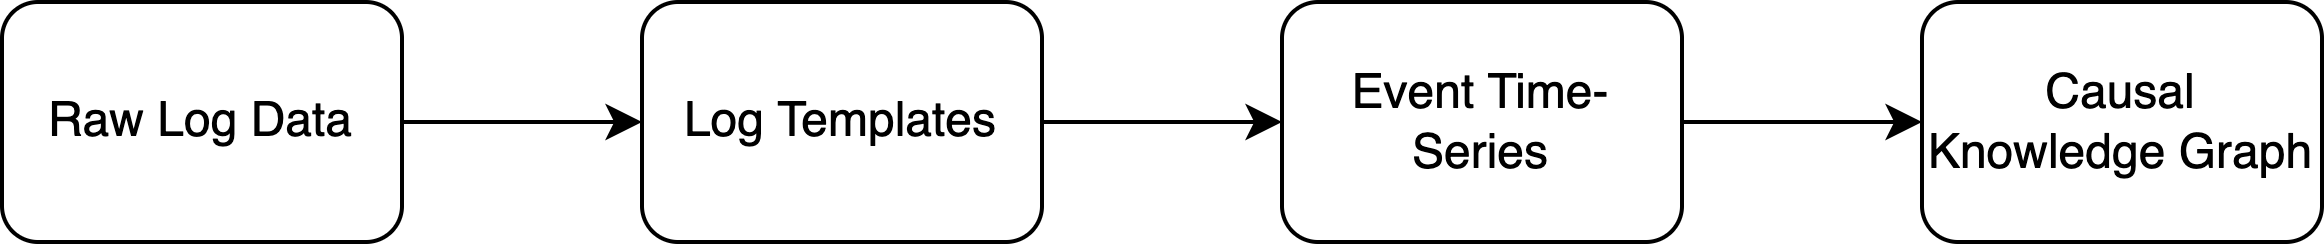
\includegraphics[width=\textwidth]{figures/structure.png}
    \caption{The general processing flow.}
\end{figure}
The overview of causal analysis literature is shown in Figure \hyperref[fig:structure]{1}. This analysis flow follows the main existing approaches \cite{jarry2021quantitative,jia2017approach,kobayashi2017mining,lou2010mining,otomo2019latent}.\newline

The input data is a set of raw log messages, including timestamp, source parameters, and free-format messages. First, we generate log templates of the log messages with some template generation algorithms to aggregate the messages into a set of event time-series in a time bin. We define a node of causal discovery as an event time-series, which corresponds to one per device per log type (log template). Some approaches also apply time-series preprocessing to remove periodicity and regularity, which causes false causality detection \cite{jarry2021quantitative,kobayashi2017mining}. Finally, we conduct causal discovery with the event time-series input to get the causal knowledge graph.